\section{Results}
\label{results}
In order to analyze the various methods described in Section \ref{Methods}, we looked at a 1D advection problem. Although we developed our code in 2D, the advection of waves in 1D highlights the similarities and differences between the methods. While we were most interested in resolving sharp discontinuities, we wanted to be sure that the method didn't artificially sharpen other types of waves. We have therefore included a square wave, a triangular wave and an exponential smooth wave in Figures \ref{First_Order}-\ref{fig:SUPG}.

\begin{figure}[htbp]
\begin{center}
\mbox{
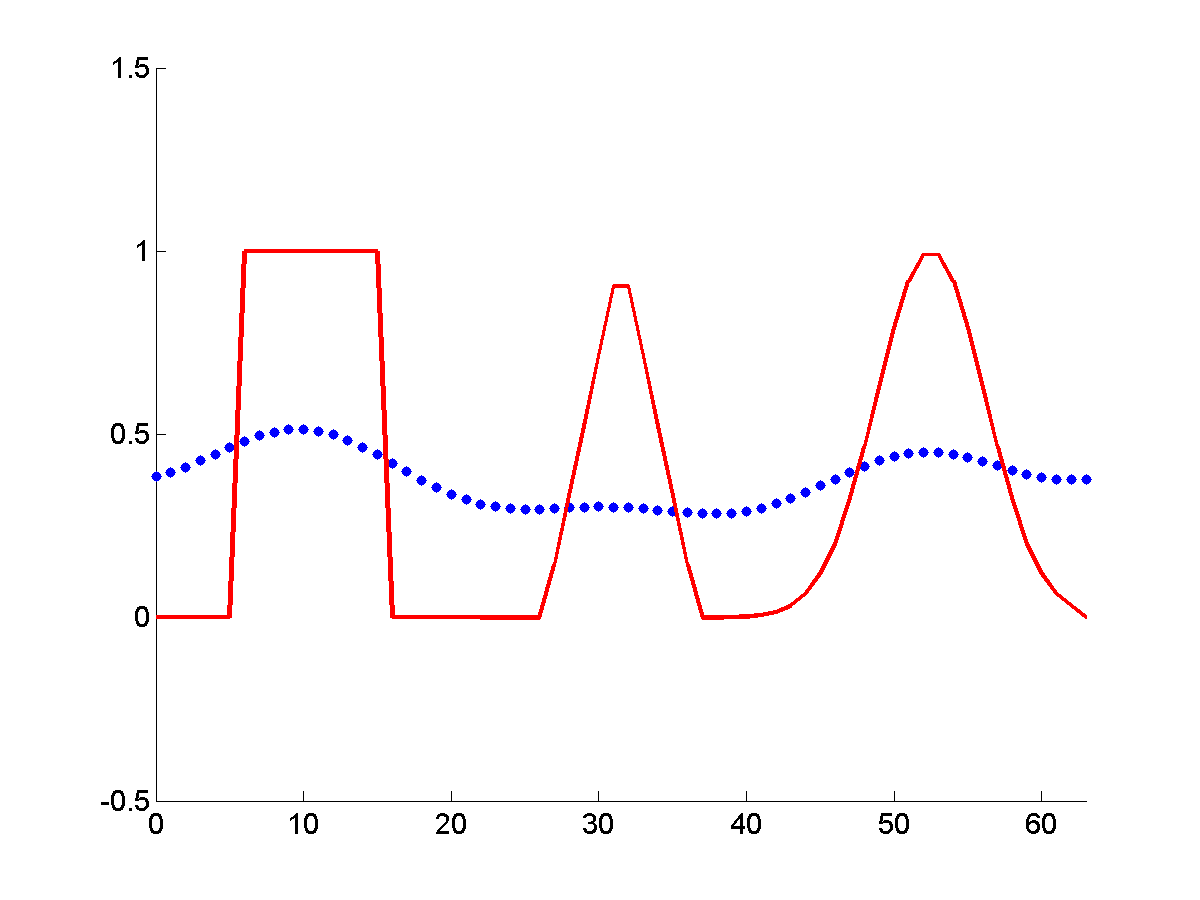
\includegraphics[width=0.31\textwidth]{Upwind_1.png}
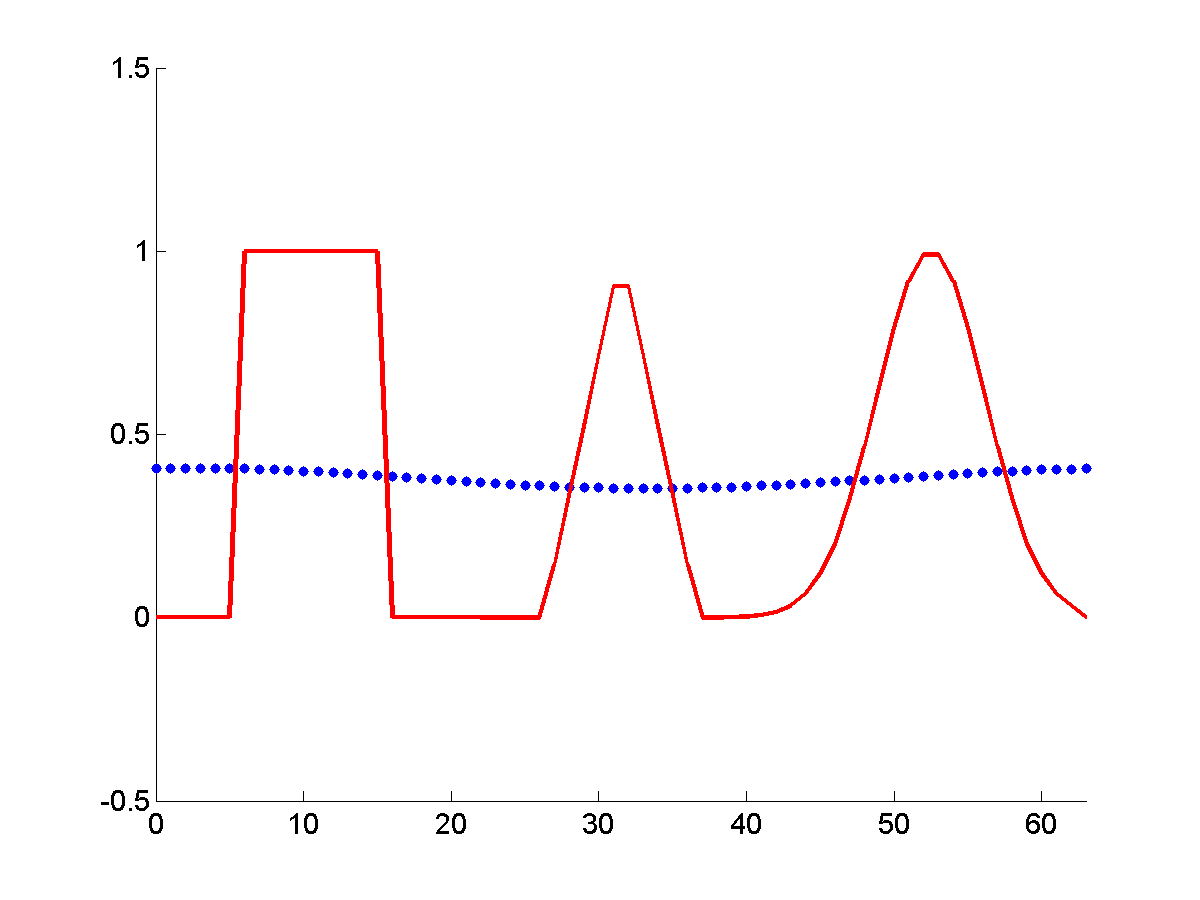
\includegraphics[width=0.31\textwidth]{Upwind_5.png}
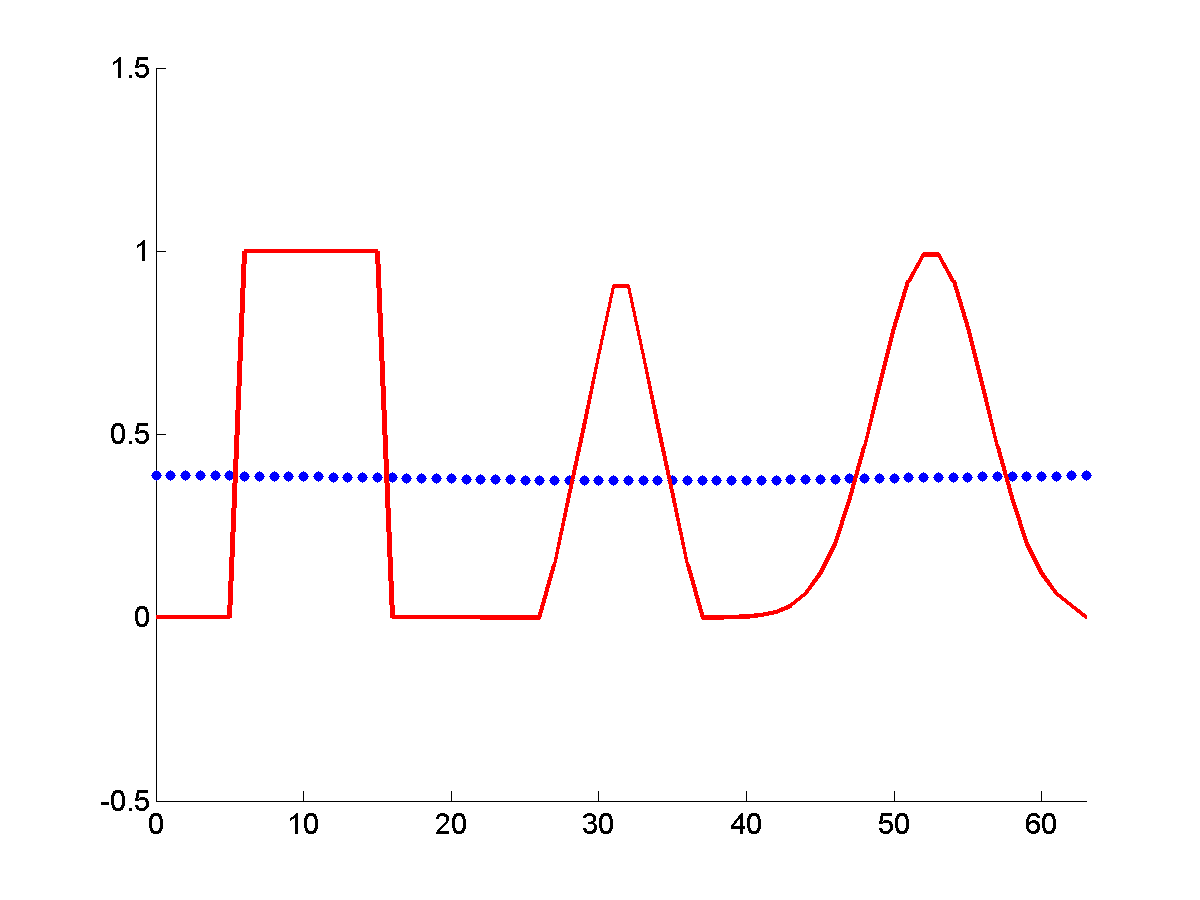
\includegraphics[width=0.31\textwidth]{Upwind_10.png}
} 
\mbox{  
\makebox[0.31\textwidth][c]{(a)}
\makebox[0.31\textwidth][c]{(b)}
\makebox[0.31\textwidth][c]{(c)}
}
\caption{Advection of a square wave, a triangular wave and an exponential wave over time with periodic boundary conditions after (a) 1 pass through the domain, (b) 5 passes through the domain and (c) 10 passes through the domain using a first order upwind method.}
\label{First_Order}
\end{center}
\end{figure}

\begin{figure}[htbp]
\begin{center}
\mbox{
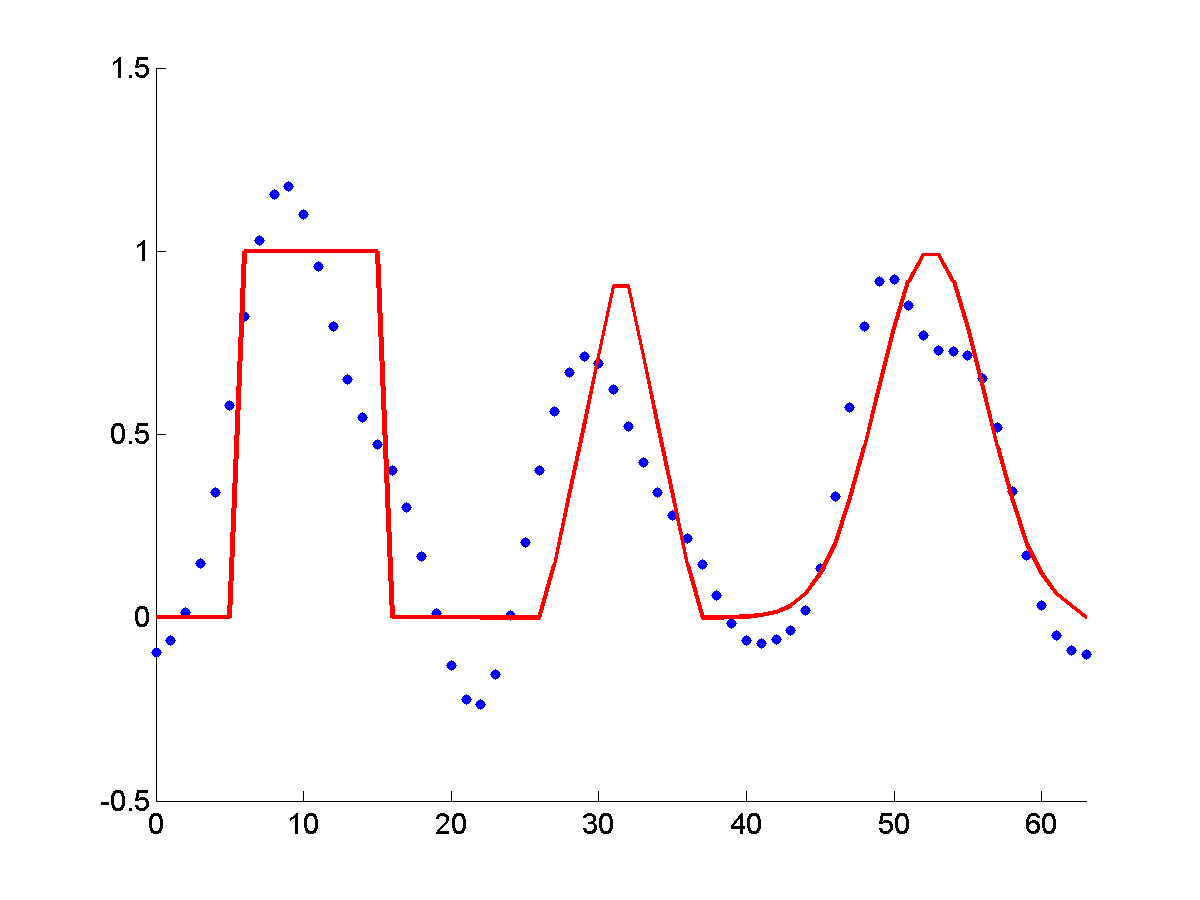
\includegraphics[width=0.31\textwidth]{Lax-noTVD_1.png}
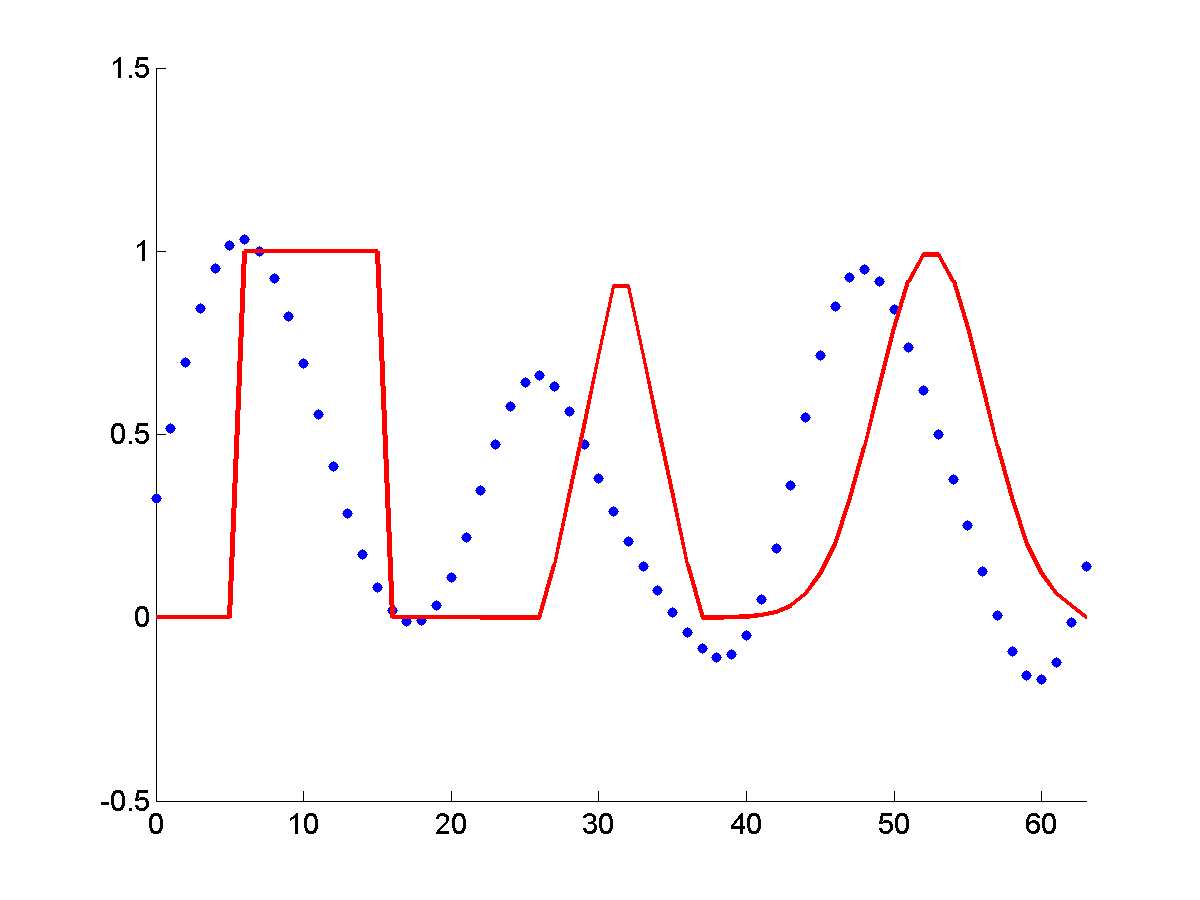
\includegraphics[width=0.31\textwidth]{Lax-noTVD_5.png}
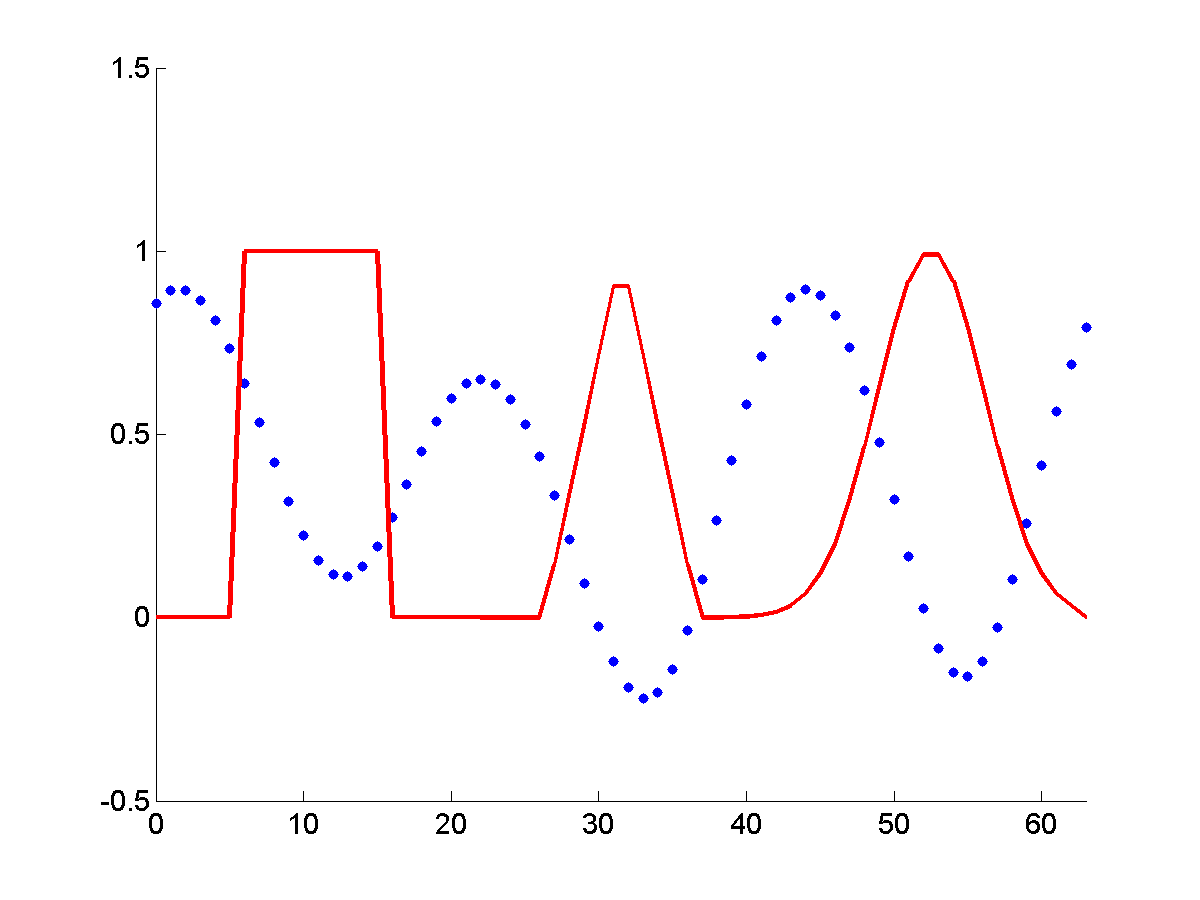
\includegraphics[width=0.31\textwidth]{Lax-noTVD_10.png}
} 
\mbox{  
\makebox[0.31\textwidth][c]{(a)}
\makebox[0.31\textwidth][c]{(b)}
\makebox[0.31\textwidth][c]{(c)}
}
\caption{Same caption as Figure \ref{First_Order} except that a Lax-Wendroff method without any slope limiters was used to advect the waves.}
\label{fig:Lax-noTVD}
\end{center}
\end{figure}

\begin{figure}[htbp]
\begin{center}
\mbox{
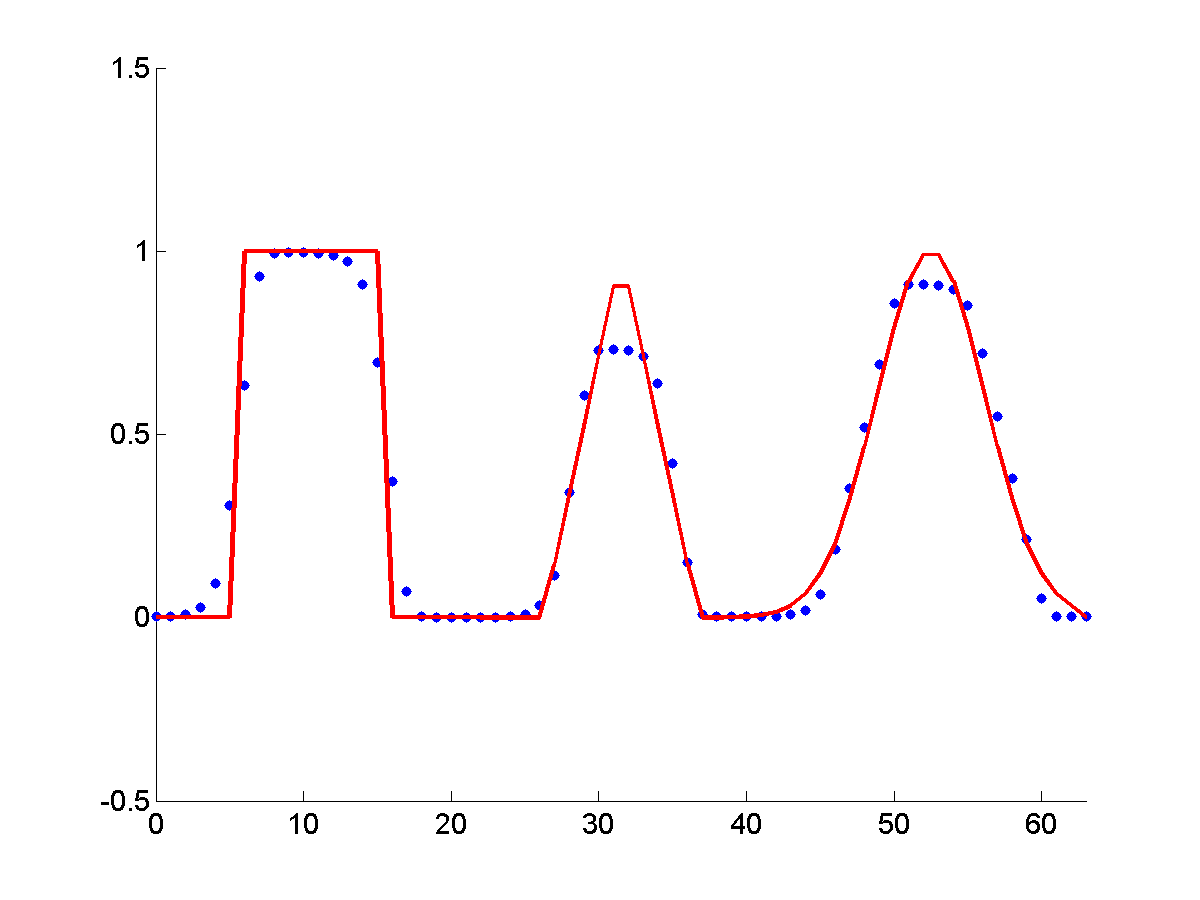
\includegraphics[width=0.31\textwidth]{Lax-wTVD_1.png}
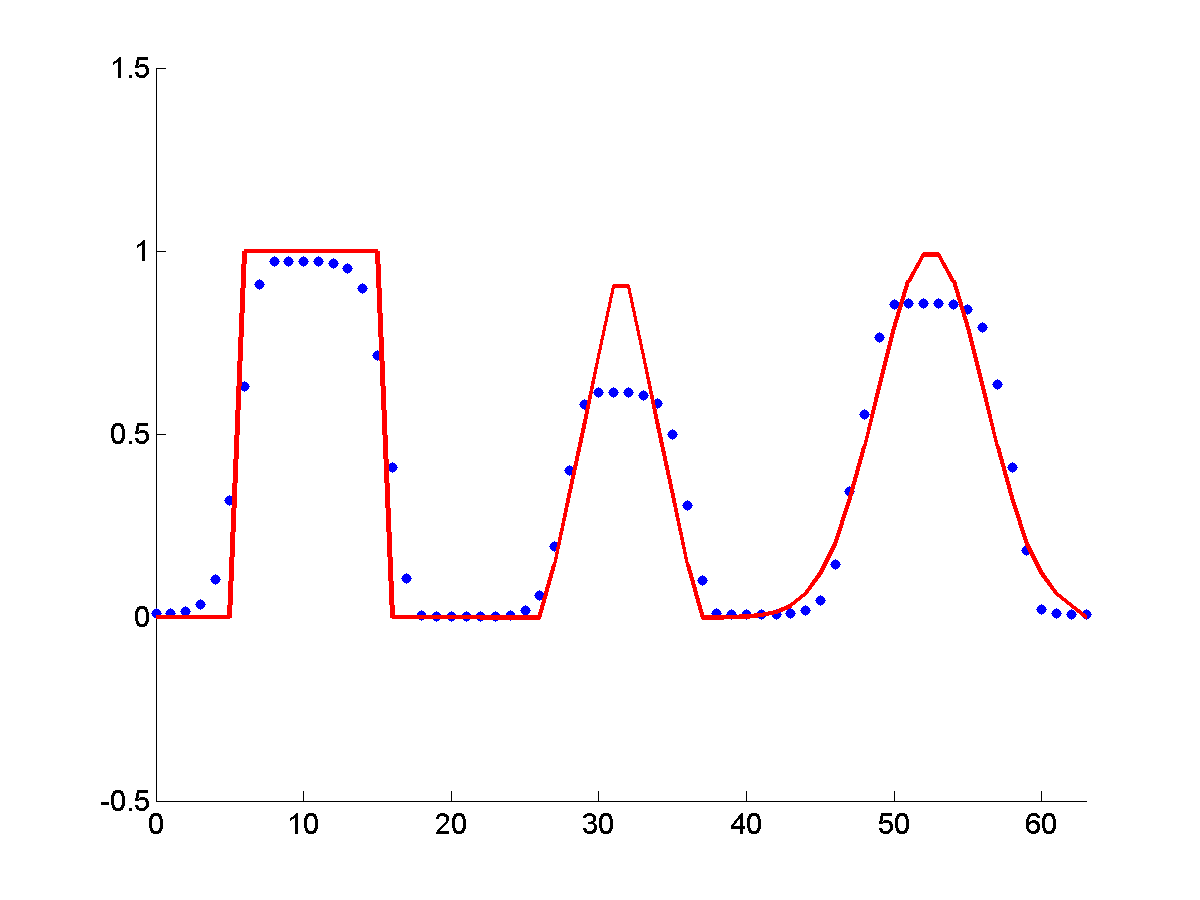
\includegraphics[width=0.31\textwidth]{Lax-wTVD_5.png}
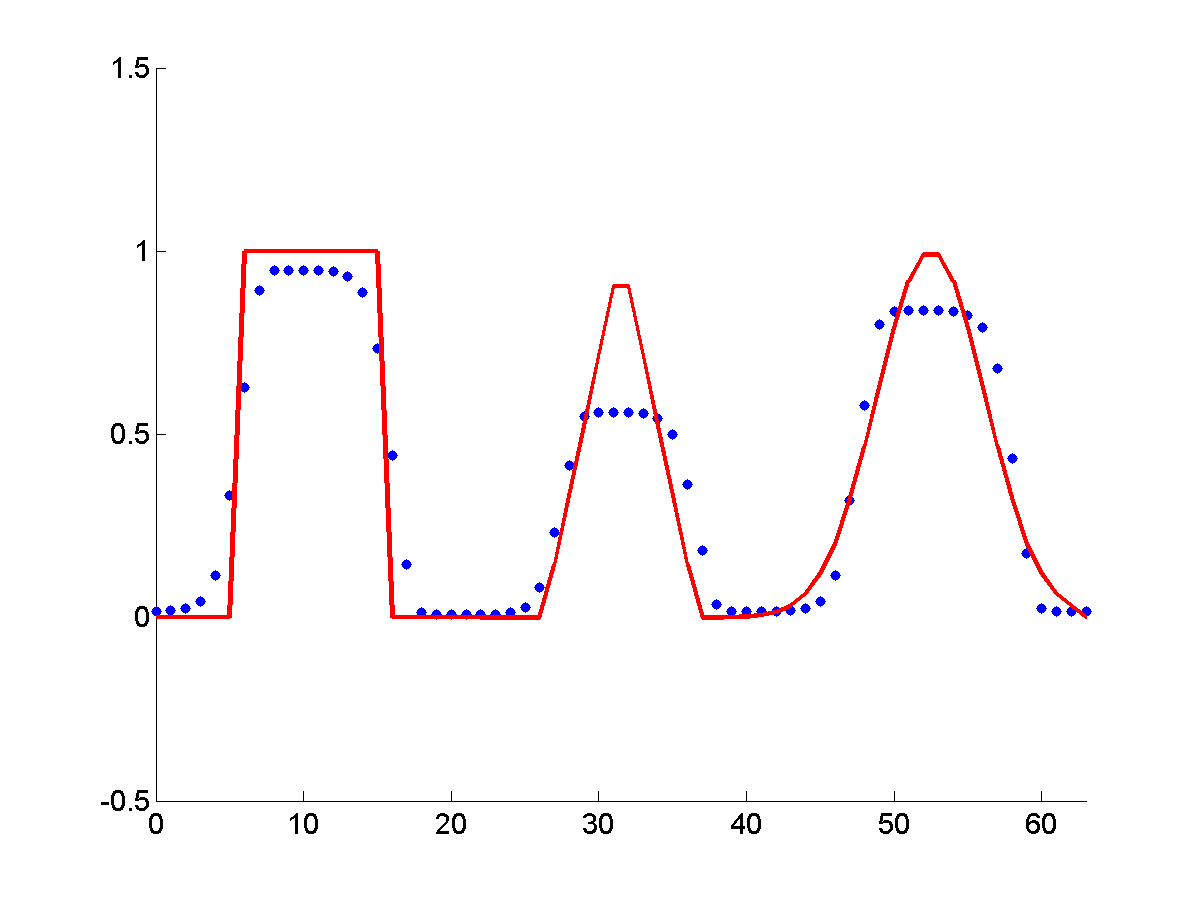
\includegraphics[width=0.31\textwidth]{Lax-wTVD_10.png}
} 
\mbox{  
\makebox[0.31\textwidth][c]{(a)}
\makebox[0.31\textwidth][c]{(b)}
\makebox[0.31\textwidth][c]{(c)}
}
\caption{Same caption as Figure \ref{First_Order} except that a Superbee Limiter was used along with the Lax-Wendroff method to advect the waves.}
\label{fig:Lax-wTVD}
\end{center}
\end{figure}

\begin{figure}[htbp]
\begin{center}
\mbox{
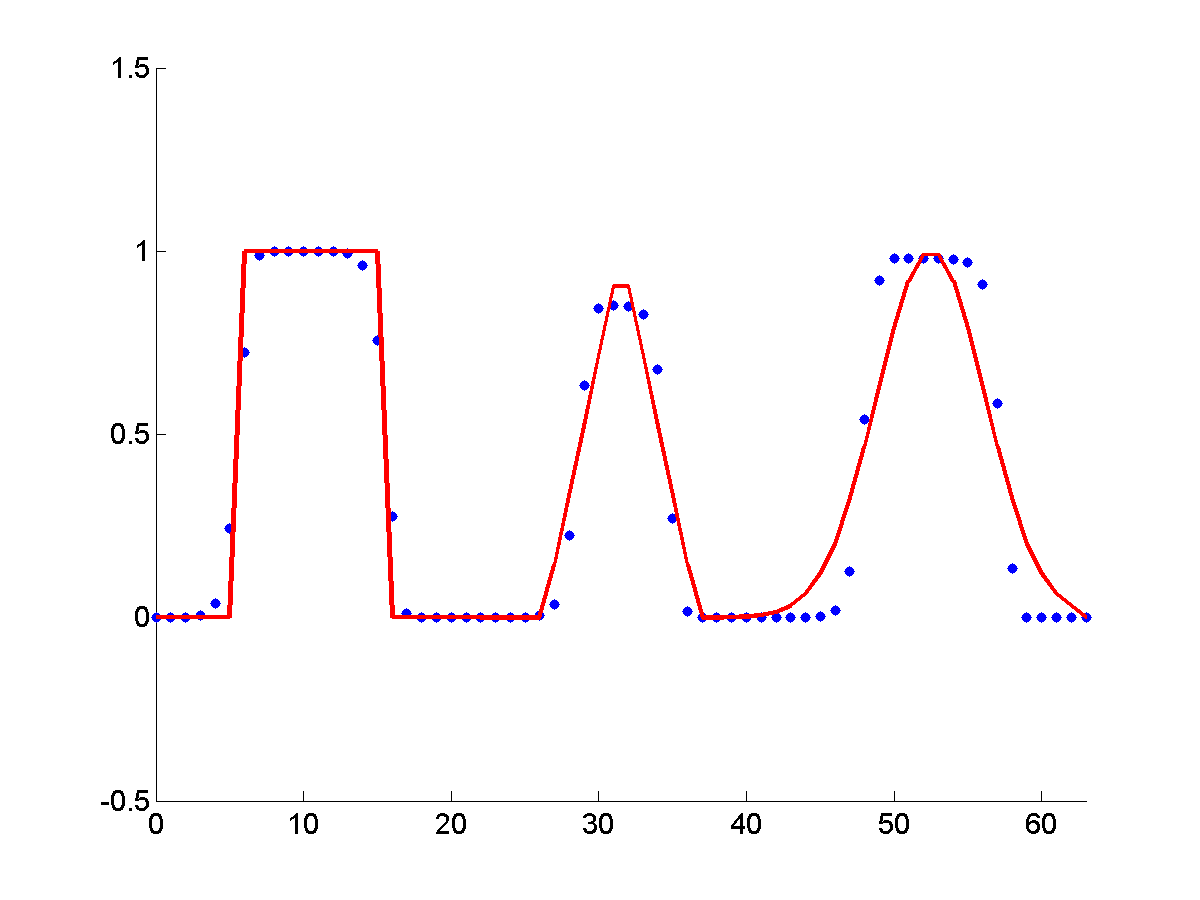
\includegraphics[width=0.31\textwidth]{MUSCL_1.png}
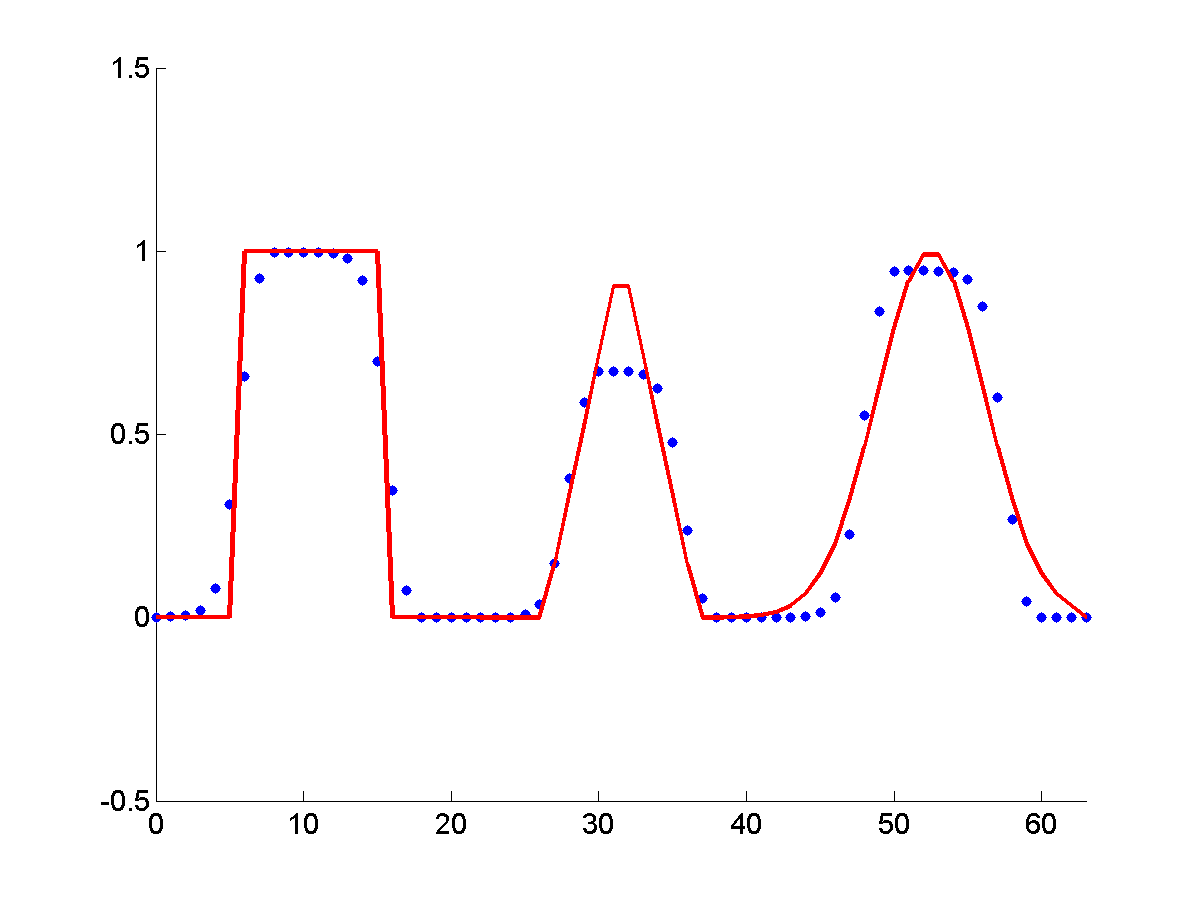
\includegraphics[width=0.31\textwidth]{MUSCL_5.png}
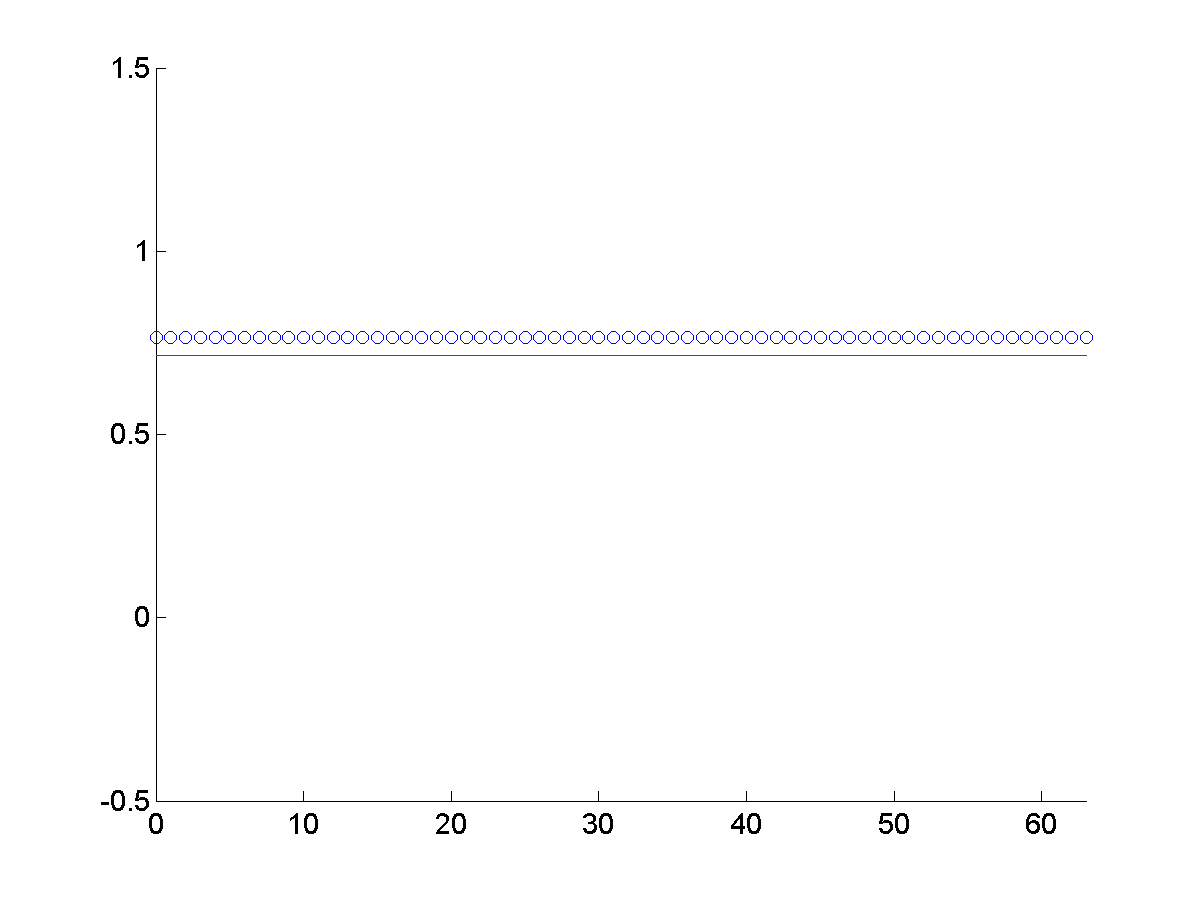
\includegraphics[width=0.31\textwidth]{MUSCL_10.png}
} 
\mbox{  
\makebox[0.31\textwidth][c]{(a)}
\makebox[0.31\textwidth][c]{(b)}
\makebox[0.31\textwidth][c]{(c)}
}
\caption{Same caption as Figure \ref{First_Order} except that a MUSCL with an ACM were used advect the waves.}
\label{fig:MUSCL}
\end{center}
\end{figure}

\begin{figure}[htbp]
\begin{center}
\mbox{
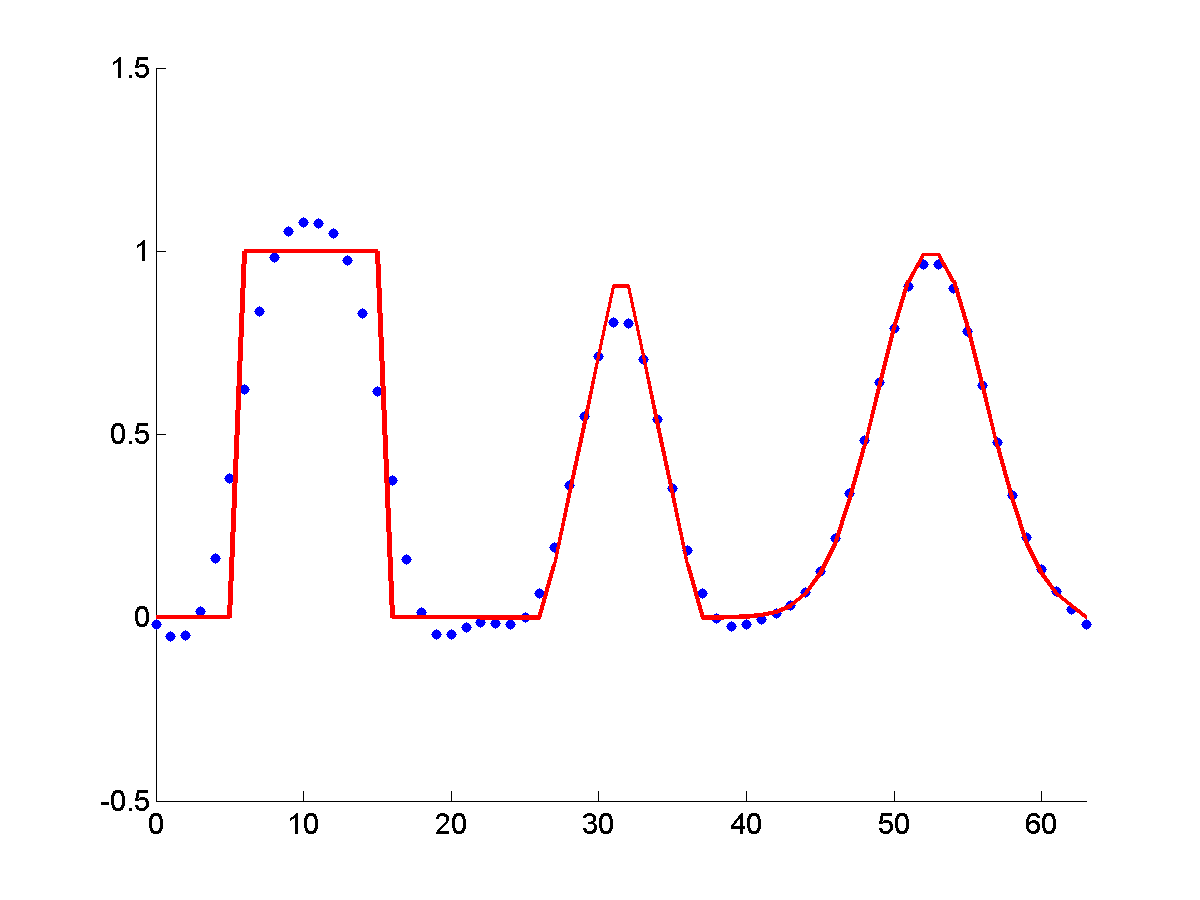
\includegraphics[width=0.31\textwidth]{SUPG_1.png}
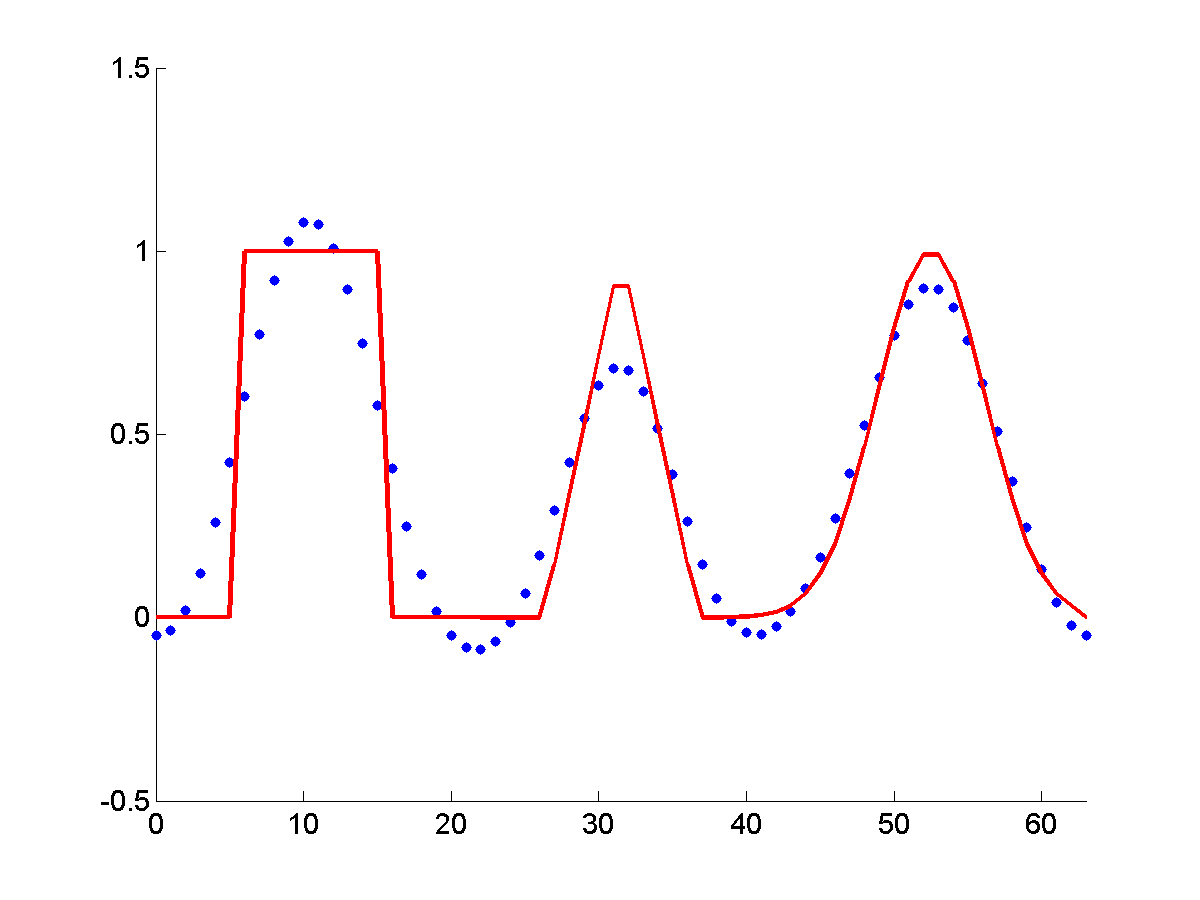
\includegraphics[width=0.31\textwidth]{SUPG_5.png}
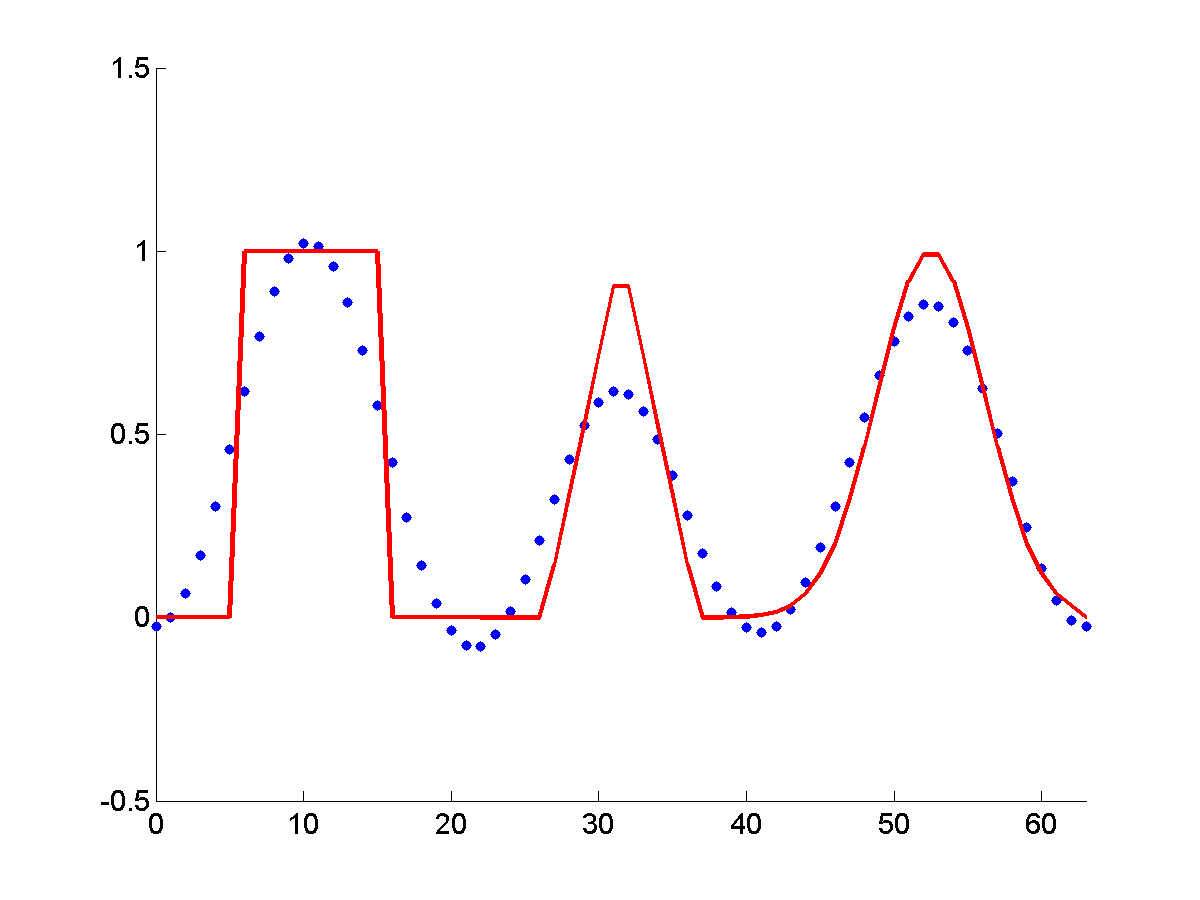
\includegraphics[width=0.31\textwidth]{SUPG_10.png}
} 
\mbox{  
\makebox[0.31\textwidth][c]{(a)}
\makebox[0.31\textwidth][c]{(b)}
\makebox[0.31\textwidth][c]{(c)}
}
\caption{Same caption as Figure \ref{First_Order} except that SUPG was used to advect the waves.}
\label{fig:SUPG}
\end{center}
\end{figure}

A graphics package called MPE is employed in the Wave Code described in Section \ref{WaveCode} to show realtime images of the desired variable. The evolution of the height in the shallow water equations as a wave moves from left to right is shown in Figure \ref{fig:H} and a passive tracer concentration is shown in Figure \ref{fig:phi} for the same time steps.

\begin{figure}[htbp]
\begin{center}
\mbox{
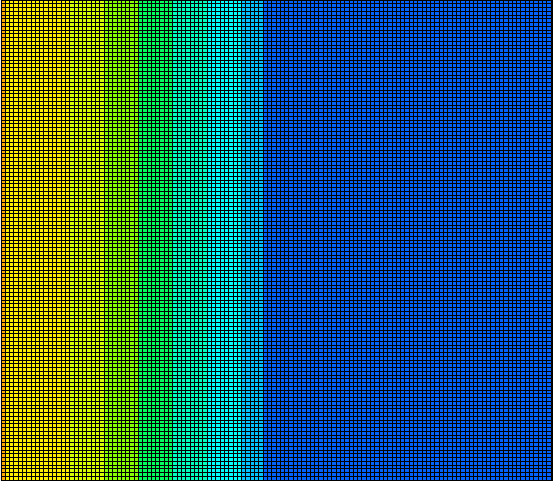
\includegraphics[width=0.31\textwidth]{H_1.png}
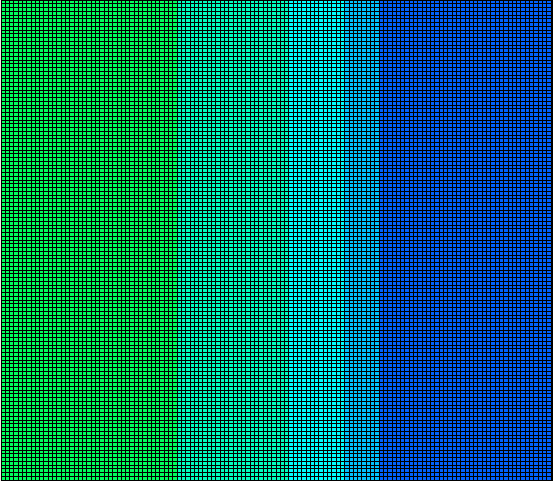
\includegraphics[width=0.31\textwidth]{H_10.png}
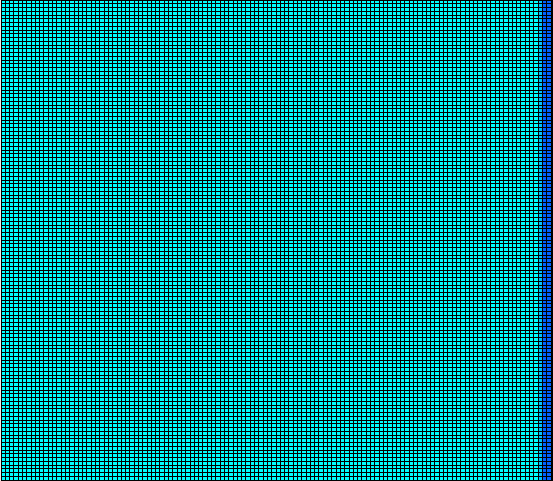
\includegraphics[width=0.31\textwidth]{H_20.png}
} 
\caption{Evolution of the height of a wave over time using the GPU enabled wave code.}
\label{fig:H}
\end{center}
\end{figure}

\begin{figure}[htbp]
\begin{center}
\mbox{
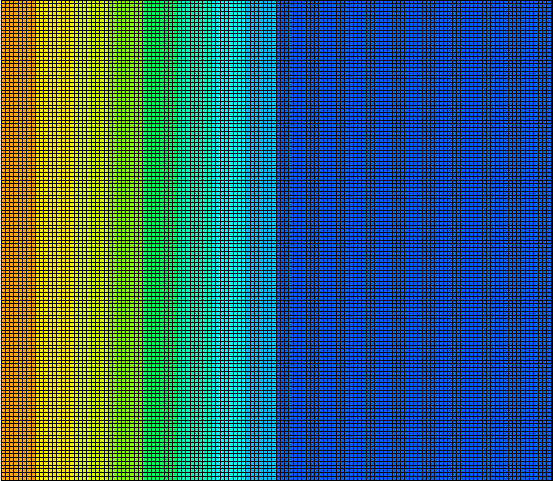
\includegraphics[width=0.31\textwidth]{phi_1.png}
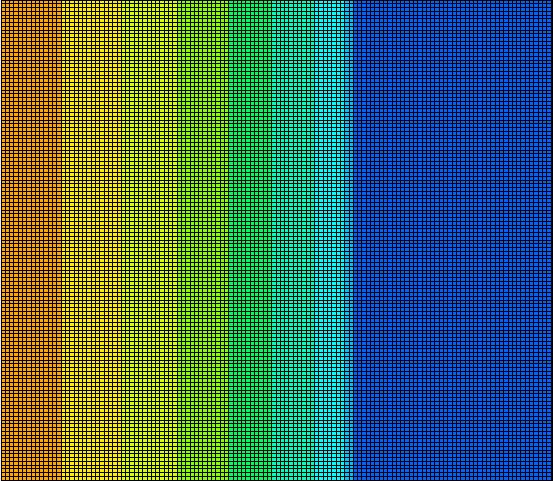
\includegraphics[width=0.31\textwidth]{phi_10.png}
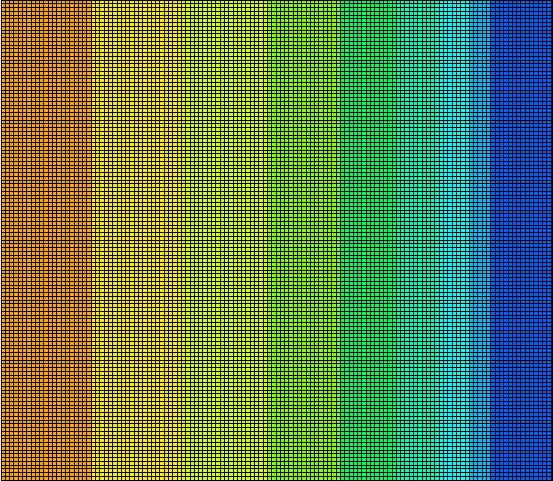
\includegraphics[width=0.31\textwidth]{phi_20.png}
} 
\caption{Evolution of the concentration of a dye over time using the GPU enabled wave code.}
\label{fig:phi}
\end{center}
\end{figure}